\chapter{Raft user study}
\label{userstudy}

This is the first of four chapters that each evaluate an aspect of
Raft:
\begin{compactitem}
\item This chapter evaluates Raft's understandability,
\item Chapter~\ref{correctness} discusses Raft's correctness,
\item Chapter~\ref{leaderelection} evaluates Raft's leader election
algorithm, and
\item Chapter~\ref{performance} discusses Raft's implementations and
evaluates its performance.
\end{compactitem}


\blfootnote{This study involved human subjects. It was
approved under exempt status by the Stanford University IRB
(Institutional Review Board) as Protocol~26663.}


We designed Raft to be understandable based on our intuitions and
anecdotal evidence, but we wanted to evaluate its understandability more
objectively. Although measuring understandability is inherently
difficult, this was important to us for two reasons. First, without an
evaluation, our central claim that Raft is easy to understand would be
hard to justify. Second, one of our goals was to propose understandability
as a first-class feature in computer systems, so we also carried the
burden of proposing a way to evaluate it.

To evaluate Raft's understandability, we conducted an experimental
study. This study compared students' ability to answer quiz questions
about Raft and Paxos after learning each algorithm. Our participants
were upper-level undergraduate and graduate students at Stanford
University and the University of California, Berkeley. We recorded
video lectures of Raft and Paxos and created corresponding
quizzes.
The Raft lecture covered the basic Raft algorithm
(Chapter~\ref{basicraft}) and briefly covered the joint consensus
approach to arbitrary membership changes
(Section~\ref{membership:arbitrary});
the Paxos lecture covered enough material to create an
equivalent replicated state machine, including single-decree Paxos,
Multi-Paxos, cluster membership changes, and a few optimizations needed in
practice (such as leader election).
The lecture videos and slides are available online~\cite{study}.
The quizzes tested basic
understanding of the algorithms and also required students to reason
about corner cases. Each student watched one video, took the
corresponding quiz, watched the second video, and took the second quiz.
About half of the participants did the Paxos portion first and the other
half did the Raft portion first, in order to account for both individual
differences in performance and experience gained from the first portion
of the study. We compared participants' scores on the two quizzes to determine
whether participants showed a better understanding of Raft than Paxos.

On average, participants scored 22.6\% higher on the Raft
quiz than on the
Paxos quiz (out of a possible \SI{60}{points}, the mean Raft score was 25.7
and the mean Paxos score was 21.0). Accounting for whether people learn
Paxos or Raft first, a linear regression
model predicts scores \SI{12.5}{points} higher
on the Raft quiz than on the
Paxos quiz for students with no prior Paxos experience.
Section~\ref{userstudy:results:quizzes} analyzes the quiz
results in detail.

We also surveyed participants after their quizzes to see which algorithm
they felt would be easier to implement or explain. An overwhelming
majority of participants reported Raft would be easier to implement and
explain (33 of 41 for each question). However, these self-reported
feelings may be less reliable than participants' quiz scores.
Section~\ref{userstudy:results:survey} analyzes the survey results in
detail.

Our study was unconventional for systems research, and we learned many
lessons while designing and conducting it.
For example, in a user study, almost all of the work must be done before
seeing any results; this leaves little room for error.
Two sections discuss the lessons we learned.
Section~\ref{userstudy:methodsdiscussion} explores the numerous design
decisions we considered in developing our methods and materials.
Section~\ref{userstudy:approachdiscussion} explores how effectively the
experiment convinced others of Raft's understandability, and
whether it was worth the time and effort we put into it.

\section{Study questions and hypotheses}

Our primary goal in the study was to show Raft's understandability. A
developer should be able to learn the Raft algorithm well enough to
produce a correct implementation, without an
unnecessary burden of time and effort. Unfortunately, Raft's
understandability is difficult to measure directly. There is no
established measure for understandability, and we have no way of telling
whether Raft is the most understandable possible algorithm.

To arrive at an experiment, we needed to formulate metrics that we could
measure and hypotheses that we could test.
We first needed a proxy
for measuring someone's understandability. We chose to quiz participants
and measure their quiz scores
(Section~\ref{userstudy:methodsdiscussion:testing} discusses an
alternative of having participants implement the algorithms instead).
Second, we needed to draw a comparison between participants' quiz scores
on Raft and on other consensus algorithms. We chose to compare Raft to
Paxos, the most popular consensus algorithm used today.

We wanted to explore the following questions in our study:
\begin{enumerate}

\item Is Raft easier to understand than Paxos?

We predicted students would score higher on the Raft quiz than on the
Paxos quiz.

\item Which aspects of Raft are hardest to understand?

We were interested in this question as it could help lead to further
improvements in Raft's understandability.
We thought students were most likely to struggle with commitment and
membership changes in Raft. We felt these were the most complex and
difficult aspects of Raft to explain, so students were most likely to
have difficulty understanding them
(this predates Raft's simpler single-server membership change
algorithm). We also felt that Paxos'
$\alpha$-based membership approach was simpler to explain (though the
secondary issues it leaves unsolved are significant).

\item How does knowing Paxos affect learning Raft, and vice versa?

We predicted that students would generally score higher on their second
quiz. We had two reasons for this. First, consensus algorithms share
fundamental concepts, and students should be able to grasp a concept
more easily when seeing it a second time. Second, since the lectures and
quizzes followed the same format, we thought students would gain useful
experience during the first lecture and quiz.

\item Do people prefer to use Raft over alternatives?

We predicted Raft's understandability would result in a preference to
implement and explain Raft.

\end{enumerate}


\section{Discussion about the methods}
\label{userstudy:methodsdiscussion}

%

Because there is little precedent for this sort of experiment in
computer systems literature, we reasoned through many our experimental
design decisions from first principles.
We are especially thankful for Scott Klemmer's valuable help during this
process.
This section explains why we arrived at our methods by
describing the alternatives we considered for each decision,
including:
\begin{compactitem}
\item Our
choice of participants and how to motivate their participation
(Section~\ref{userstudy:methodsdiscussion:participants}),
\item
How to teach the algorithms to the participants
(Section~\ref{userstudy:methodsdiscussion:teaching}),
\item
How to test their understanding
(Section~\ref{userstudy:methodsdiscussion:testing}),
\item
How to evaluate their performance
(Section~\ref{userstudy:methodsdiscussion:grading}),
\item
What questions to ask in the survey
(Section~\ref{userstudy:methodsdiscussion:survey}),
and
\item
How to discover and fix problems in the study before starting
(Section~\ref{userstudy:methodsdiscussion:pilots}).
\end{compactitem}
The methods we ultimately decided to use are then presented in
Section~\ref{userstudy:methods} in a more formal APA
(American Psychological Association) style.

One common principle we applied was to test participants at the start
of the learning curve for the algorithms. We wanted to see how easily
they could move from no knowledge to a moderate level of understanding.
While we hoped that our participants would gain at least a basic
understanding of both algorithms, we did not
want to over-prepare them. Given infinite time, most participants will
eventually understand any consensus algorithm. Thus, to measure a
difference between algorithms, we had to test participants at the
start of the learning curve. For example, this meant we faced a tension
in motivating participants, as discussed in the next subsection: we
wanted them to try, but we did not want them to study the algorithms
extensively.

\subsection{Participants}
\label{userstudy:methodsdiscussion:participants}

We invited students from both Stanford and Berkeley to participate in our
study. This both
increased our sample size and broadened the generality of our results. We
chose to use the same materials and procedures in both schools so that
we could compare participants' performance across schools.

We considered various ways to use course grades to incentivize students
to participate in the study. We wanted students to put equal effort into
learning each algorithm, and we only wanted them to watch the lectures
to prepare (without using outside information or studying excessively).
Unfortunately, we had substantial
concerns for each approach we considered to incentivize students:
\begin{itemize}
\item If students' participation affected their course grades but they
earned credit for even incorrect answers, we were concerned that
students might not pay attention to the lectures. For example, a student
who skipped the lectures but filled in the quizzes with any answer that
came to mind would still receive full credit towards his/her course grade.
\item If students' scores on their quizzes affected their course grades,
we were concerned that students might spend too much time preparing for
the quizzes or that they might work harder on the more difficult to
understand algorithm in
order to earn the same grade. We wanted to test participants at the
start of the learning curve; we didn't want students to understand the
algorithms so well that our questions could measure no difference in
understanding between the algorithms. We also wanted them to spend equal
effort on each algorithm.
\item If students were awarded extra course credit for participation or
for good quiz scores, we were concerned that poorly performing or more
stressed students might be overrepresented in our participants.
\item Another idea we considered was to award students all of the course credit 
for scoring at least 50\% on \emph{either} quiz. Our
concern with
this approach was that it would leave too many possible explanations for
quiz scores. For example, would students stop after their first
algorithm if they believed they did well enough? Would students choose
ahead of time to try to do well on Raft and not worry about the Paxos
quiz (or vice versa)?
\end{itemize}

For the Stanford students, we ultimately decided to give full course
credit (5\% of the total course grade)
for reasonable participation in the study. We intentionally left
this definition vague, but if a student appeared to put some effort into
the study, we awarded them full course credit. The students were also
informed that the material might show up again on the course's final
exam. Almost every student in the Stanford class participated (see
Table~\ref{tab:userstudy:participation}).

However, the only incentive for the Berkeley participants was the
opportunity to learn the material.
The instructors for the Berkeley class chose not to factor study
participation into the course grades, and the class did not have exams.
Even without additional incentives, at least one third of the students
in the Berkeley class
participated (see Table~\ref{tab:userstudy:participation}).

\begin{table}
\centering
\begin{tabular}{lrrrrc}
school & total & \ $\geq$ one quiz & \ $\geq$ both quizzes & full study
& incentive \\
\hline
\noalign{\vskip .75ex}
Stanford & 34 & 33 & 31 & 31 & 5\% part.\ grade, final exam \\
Berkeley & 46 & 16 & 12 & 11 & none \\
Total    & 80 & 49 & 43 & 42 & - \\
\end{tabular}
\vcaption[study participation]{
Study participation.
The ``total'' column lists the number of students in each class;
the ``$\geq$ one quiz'' column lists the number that completed at least
one quiz;
the ``$\geq$ both quizzes'' column lists the number that completed at least
both quizzes;
and
the ``full study'' column lists the number that completed
both quizzes and the survey.
\\
The total number of participants is approximate. For Berkeley, this
number is based on the course email list and is likely an over-estimate
(only 25 students signed up to do the homework towards the end of the
course).
}
\label{tab:userstudy:participation}
\end{table}

\subsection{Teaching}
\label{userstudy:methodsdiscussion:teaching}

We had many options in how to teach the algorithms to the participants.
Not only are there many ways to teach in general, but there are also
various approaches to teaching Paxos in particular. Our goal in the
study was to compare the algorithms, not the ways they were conveyed.
Therefore, it was important for the teaching method and style to be
consistent. We wanted to convey the algorithms in similar ways, and we
wanted to cover equivalent content.
We also wanted participants to spend no more than a few hours per
algorithm. We thought this would be reasonable to ask of our
participants, and we would then be able to test them at the start of the
learning curve for each algorithm.

We considered using papers to teach our participants, but this had two
problems.
First, we could not find a suitable Paxos paper. This paper would have
had to:
\begin{compactitem}
\item Cover a relatively understandable variant of Paxos (there is no
single agreed upon Paxos algorithm, but some are easier to understand
than others);
\item Describe it completely enough to build a replicated state
machine;
\item Be accessible to students with no background in the topic,
without needing to understand related work first; and
\item Be of similar quality, style, and length to the Raft paper.
\end{compactitem}
We could have written such a paper, but it would have taken months.
The second problem is that papers take many hours to read,
and we wanted the participants to be able to learn
the algorithms in less time.

Instead, we decided to teach the participants through lectures. We
estimated that we could cover enough material for each algorithm in a
one-hour lecture. This was short enough that it didn't unduly burden
our participants, yet it was long enough to cover a significant amount of
material at a comfortable pace. It was also short enough that we
could still quiz participants towards the start of the learning curve
for the algorithms.

We chose to have John Ousterhout give the lectures for both algorithms,
rather than using a different lecturer for Paxos. In trying to maximize
consistency across the algorithms, we considered the following factors
in our decision:
\begin{itemize}
\item \textbf{Expertise:} We wanted an equivalent level of expertise on
each algorithm, and we didn't consider ourselves experts on Paxos before
the study. We could have brought in an expert on Paxos to give the Paxos
lecture. Instead, Ousterhout based his slides on those of experts, and
in preparing for the Paxos lecture, we believe we learned Paxos well
enough to consider ourselves sufficiently knowledgeable in it.
\item \textbf{Teaching style and ability:} Ousterhout was able to keep
this very consistent across his two lectures, whereas we might have
struggled with different teaching styles and abilities if a separate
lecturer gave the Paxos lecture.
\item \textbf{Lecture quality:} Ousterhout giving both lectures raises
concerns that he might not have put in the effort to produce an equally
good Paxos lecture. However, he tried to produce equivalent lectures,
and this is mitigated by basing his Paxos slides off of those of
experts. (Also, the Raft lecture had known deficiencies during the
study: we made some last-minute changes to fix a bug in it that could
have been clearer if we had more time. Moreover, it presented the more
complex form of membership changes, as it predated the simpler
single-server change algorithm.)
Balancing lecture quality might
have been more difficult with a different Paxos lecturer, since the
second lecturer may not have been as committed to the study.
\end{itemize}


We wanted to teach a variant of Paxos that was relatively
understandable and complete, while staying true to the fundamentals of Paxos.
Unfortunately, there is no agreed upon variant of Paxos; different
instructors disagree on which variant to teach.
We ultimately settled on a variant from David Mazi\`eres~\cite{dmpaxos},
which is not only efficient but also relatively understandable.
However, we used Leslie Lamport's $\alpha$ approach~\cite{Lamport:2001} to
reconfiguration rather than Mazi\`eres's. Although Lamport's approach has the
undesirable property that it limits Paxos's concurrency during normal
operation, we (including Mazi\`eres) believe its basic idea is easier to
understand than Mazi\`eres's and other approaches.

We recorded both lectures on video rather than having John Ousterhout
present them in person. There were several advantages to recording them:
\begin{compactitem}
\item We could fit more material in the same amount of time, since we
could re-record segments when we made mistakes.
\item We were able to debug problems with our lectures during the two
pilot studies we ran for each algorithm
(see Section~\ref{userstudy:methodsdiscussion:pilots}).
Having them recorded allowed us to catch issues and fix them reliably.
\item Participants could watch the lectures in different orders and
still see the same exact material.
\item Students could watch the lectures at their own pace and at their
own schedule. They could re-watch segments or speed up and slow down the
videos as they wished. We did not enforce time limits on the lectures,
so students could watch them at their own pace.
\item The video lectures remain as documentation for the study and could
be used in a repeated study. Other people outside the study have also
used the videos to learn the algorithms on their own
(our Raft lecture has \num{14480} views on YouTube as of August 2014,
and our Paxos lecture has \num{9200} views).
\end{compactitem}
A possible disadvantage is that students could not ask questions during
the lectures. On the other hand, questions would have disrupted the
consistency benefits of having recorded lectures. For example, questions
could lead to more material being presented in one lecture than another
and could introduce additional differences between the Stanford and
Berkeley groups. We also do not know
how the recorded lectures affected study participation; while our
Stanford participation was high, it's possible that
we could have gotten higher participation at Berkeley by scheduling the
lectures in class.

We attempted to keep the video lectures fairly impersonal to reduce
bias. For example, the video components only showed the lecture slides
and not John Ousterhout himself. However, even Ousterhout's voice-over may
have been subtly biased (though he tried not to be). Concerned readers
should review the lecture videos to decide for themselves; we do not
know of any formal techniques to measure or reduce such bias.

In addition to the video lectures, we provided participants with minor
additional materials for their preparation (lecture notes and algorithm
summaries). We discouraged participants from learning about the
algorithms on their own (for example, by reading papers), but we felt
that some additional materials to review before the quiz and to reference
during the quiz would be helpful for the participants. We made copies of
the lecture slides available for easier reference, and we provided
participants with algorithm summaries in the form of a (condensed)
one-page summary for Raft and a (sparse) 3.5-page summary for Paxos.
These are included in Appendix~\ref{appendix:userstudy:supporting}.


\subsection{Testing understanding}
\label{userstudy:methodsdiscussion:testing}

A key challenge of this study was how to measure participants'
understanding of the algorithms.
%
We considered having participants implement the algorithms, which would
allow us to measure their ability to build working systems more
directly. If feasible, this approach would have been better than the
quizzes. However, we chose not to do
this because of numerous challenges. First, we estimate that implementing
significant portions of Raft or Paxos would take most experts weeks. If
we asked this of our participants, surely we would not have had so many,
and we might not have been able to draw statistically significant
conclusions. Moreover, peoples' ability to develop systems varies
greatly, so to draw statistically significant conclusions, such a study
would need large sample sizes or would need each participant to
implement both algorithms. Both options would be difficult in practice
because of the time commitment required of participants. Even if the
participation problems were solved, it would still be challenging to
measure implementations against each other. A thorough treatment would
need to include metrics of correctness, code complexity, and cost, all
of which are challenging to measure.

Instead, we chose to quiz participants to measure their understanding.
This required less time of our participants. As a result, we were able
to have each participant learn both algorithms, which
made it easier to factor out individual differences in learning and
test-taking abilities. Moreover, it was easy to compare
participants' performance based on their numeric quiz scores.

Our most difficult challenge in developing the quizzes was how to make
them fair. We first considered using questions that
applied equally to both algorithms, but such questions tended to be
too obvious for one of the algorithms because it more directly covered
the topic. Instead, we only used similar questions if the
difficulty would also be similar.

We used the following strategy to make the quizzes fair. First, we
categorized each question by difficulty:
\begin{compactitem}
\item Easy questions were essentially recall: the answer could be found in the
lecture with little or no inference. We expected students to
answer nearly all of these correctly.
\item Medium questions required the participant to apply an algorithm found in
the lecture, but it should have been straightforward to determine which
steps to apply.
\item Hard questions required the participant to figure out what rules to
apply, combine them in new ways, and/or extrapolate beyond the lecture
material. We expected that few students would be able to
answer these questions perfectly.
\end{compactitem}
Questions in the same difficulty category should require about the same
amount of inference and extrapolation from the lecture material.
We (re-)categorized questions after the lectures were created in order
to ease concerns of ``teaching to the quiz''.

Second, we assigned point values to each question based on how long we expected
it to take. The point values were intended to reflect how many minutes
it would take a reasonably prepared student to answer the question,
based on John Ousterhout's teaching experience. For example, a question that was
expected to take about five minutes was worth five points.

Third, we balanced the quizzes in categories and points. Each quiz
contained \SI{4}{points} of easy questions,
\SI{26}{points} of medium questions, and
\SI{30}{points} of hard questions.
We also compared the questions from each
quiz side-by-side to confirm that they seemed equally difficult.

We believe the quizzes we produced this way are similar in
difficulty, though we have no way to know for sure. We ask readers to
decide for themselves by reviewing the quizzes found in
Appendix~\ref{appendix:userstudy}.

Most of the questions required open-ended short answers. We also
considered using multiple choice questions, which would have been easier
to grade objectively. However, we decided on the open-ended format
because we feel it more effectively tests participants' understanding,
as it is less suggestive of responses.

The quizzes were limited in time so that participants were unable to
become experts on the questions. We did not want to give them enough
time to attempt the questions, watch the entire video again, and then
revise the answers.

In order to extract the most information from the quizzes, we made them
intentionally difficult. For example, we didn't want any participants to
earn a perfect score because then we wouldn't have been able to
distinguish differences between them. However, we later determined that
we made the quizzes a bit too hard: the maximum score was only 46.5 out
of 60. For example, most students earned 0 points on question 8 on
each quiz; had we made those questions easier, we might have been able
to better distinguish the differences between those students.

\subsection{Grading}
\label{userstudy:methodsdiscussion:grading}

We graded the quizzes using two passes. The initial (preliminary)
grading pass was more subjective, assigning grades based on perceived
understanding. The second (final) pass assigned
grades more objectively. The following steps summarize our
procedure:
\begin{compactenum}
\item Diego Ongaro and John Ousterhout created a plausible rubric.
\item Ongaro graded the quizzes fairly quickly (grading all participants
for a given question at a time in random order, alternating between
Paxos and Raft between each question).
\item Ongaro and Ousterhout revised the rubric based on problems that
arose.
\item Ongaro regraded the quizzes more carefully (grading all
participants for a given question at a time in order of
their preliminary scores, alternating between Paxos and
Raft between each question).
\end{compactenum}
The final grading rubrics are included in Appendix~\ref{appendix:userstudy}
along with the quiz questions.

We awarded partial credit in order to gain the most information from the
quiz scores as possible. For example, a blank response demonstrates no
understanding, whereas one that is on track to an answer demonstrates
some understanding; we wanted to distinguish these cases. We tried to
award points proportional to the understanding that the participant
demonstrated in his/her answer.

There are two things we could have done better. First, we exposed
ourselves to preliminary scores and results prior to completing the rubric and
adjusting the grading. It
would have been safer to avoid this, since it raises concerns that we
might have, for example, awarded fewer points to Paxos answers during the
second round of grading if we thought it was going to be a close call.
Although we question this aspect of our procedure, it is not too
worrisome because the grades and overall results and conclusions
were essentially the same after the second pass of grading. 
For example, the Raft mean was 25.74 after the preliminary pass of
grading and 25.72 after the final pass; the Paxos mean was
20.77 after the preliminary pass, then corrected to 20.98.

Second, we graded the quizzes ourselves, and this may have introduced
bias, since we hoped that the study would show that Raft is easier to
understand than Paxos. We graded ourselves because it
takes expertise in the algorithms to develop rubrics and grade responses
(which sometimes vary greatly from each other). Therefore, it was
easiest for us to do these tasks ourselves. However, we could have hired
impartial graders to confirm our grading using our rubric.


\subsection{Survey}
\label{userstudy:methodsdiscussion:survey}

We initially considered asking participants whether they understood Raft
better than Paxos, rather than quizzing them. We were informed that such
a survey would not be very reliable on its own. For example,
participants might respond favorably towards Raft if they believe that
is our desired outcome (\emph{social desirability bias}), or they may be affected by
wording in the questions. Although we settled on quizzes
for our primary results, there is still some value in
asking participants for their opinions, so we included a short survey
for participants to fill out after their second quiz.

Our survey included six questions using five-point scales (\emph{Linkert
items}) and one open-ended question for general feedback or comments. We
tried to keep the survey short to encourage participation, and the
answers were easy to collect and quantify this way.

\subsection{Pilots}
\label{userstudy:methodsdiscussion:pilots}

One challenge with this type of study is that it is very costly if
things go wrong and the study needs to be repeated. To mitigate this
risk, we attempted to discover and iron out problems with our materials
and procedures before launching the study. Thus, we conducted two pilot
studies, each with two to four volunteer participants who were not part
of the normal study.
We included \SI{90}{points} of questions on each of
the pilot quizzes; that way we could try more questions than we intended
to keep and would have the option to throw out bad questions
(our pilot quizzes included more easy questions than the final quizzes,
but we cut most of them to shorten the quizzes).
We corrected many
problems with the lectures and quizzes during the pilots, and we
feel that the pilot process was essential to the study's success.

\section{Methods}
\label{userstudy:methods}

This section describes the methods of the Raft user study in a more
formal APA
(American Psychological Association) style. It includes many technical
details that are less conceptual in nature than the topics discussed in
Section~\ref{userstudy:methodsdiscussion} but are nevertheless important
to the study.

\subsection{Study design}

The experiment employed a \emph{within-subjects} design in which each
participant was quizzed on both the Paxos and the Raft algorithms. To
account for ordering effects, it was also \emph{counterbalanced}: about
half of the participants learned Paxos and took the Paxos quiz, then
learned Raft and took the Raft quiz; the other half learned Raft and
took the Raft quiz, then learned Paxos and took the Paxos quiz.

There were two key independent variables:
\begin{compactitem}
\setlength{\itemindent}{2em}
\item Which algorithm (Paxos or Raft)?
\item Which order (Paxos then Raft, or Raft then Paxos)?
\end{compactitem}

We recorded two additional independent variables, though we hoped their
effects would be minor:
\begin{compactitem}
\setlength{\itemindent}{2em}
\item Which school did the participant come from (Stanford or Berkeley)?
\item Did the participant have prior experience with Paxos?
\end{compactitem}


\subsection{Participants}

We invited students from Stanford and Berkeley to participate in our
study. Table~\ref{tab:userstudy:participation} summarizes the
participation from each group and how many participants completed each
portion of the study.

The 33 Stanford participants were recruited from the Advanced
Operating Systems (CS240) course at Stanford University offered January
through March 2013 and taught by David Mazi\`{e}res. The students were
upper-level undergraduate and graduate students, and a small
number of remote professional students (SCPD). They were informed that
``reasonable participation'' in the study would award them
5\% of their
course grade. (They were also offered an alternate option should they
choose not to participate in the study.) They were also informed that
questions on the material may reappear on the final exam for the course.

The 16 Berkeley participants were recruited from the Distributed
Computing (CS294-91) course at the University of California, Berkeley
offered January though May 2013 and taught by Ali Ghodsi. The students
were mostly graduate-level (though at least one undergraduate student
took the course). It was vaguely suggested to the students that they
should participate in the study as part of the course, but there was no
explicit incentive to encourage participation.

\subsection{Materials}

Participants gained access to materials for the study though a
password-protected website.
The website allowed participants to proceed with the study at their own
pace and at any time of day. The various materials available on the
website are explained in more detail next.

\subsubsection{Lectures}

\begin{figure}
\centering
\fbox{
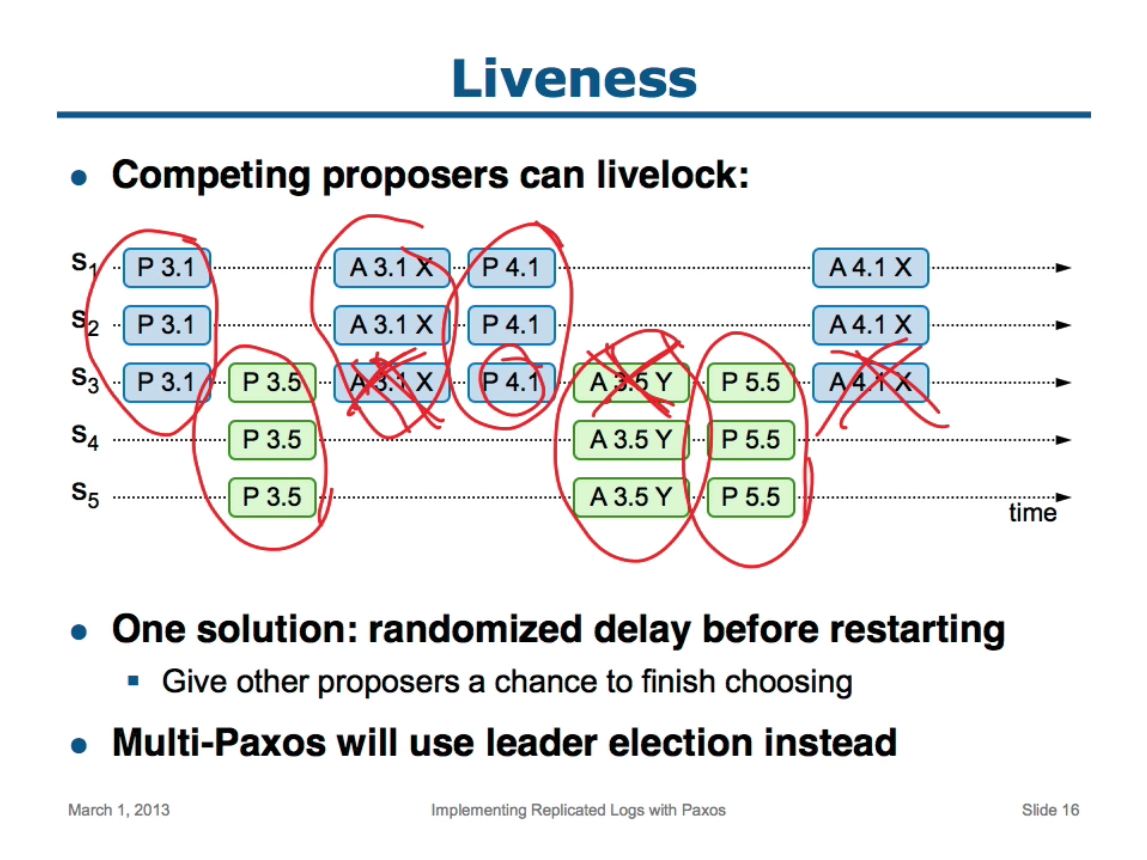
\includegraphics[scale=.5]{userstudy/stylusoverlay}
}
\vcaption[example lecture slide with stylus overlay]{
Example lecture slide marked up with stylus overlay. This slide comes
from the Paxos lecture (it shows liveness problems that could arise if
two competing proposers were too synchronized).
}
\label{fig:userstudy:stylusoverlay}
\end{figure}

Each algorithm had a corresponding video lecture. The lecture slides
were designed and created by John Ousterhout. The Paxos lecture
borrowed from slides by Lorenzo Alvisi, Ali Ghodsi, and David
Mazi\`{e}res; the Raft lecture was based on a draft of a paper
describing Raft.
The slides were made available
to the participants on the study website in both Microsoft PowerPoint
and PDF formats. The videos used a ``screencast'' format: the video
components showed only the slides and a stylus overlay, and the audio
component consisted of Ousterhout verbally explaining the slides.
Figure~\ref{fig:userstudy:stylusoverlay} shows an example of a slide with the
stylus overlay.
The
videos were recorded in advance so that students in both ordering groups
could use the same exact videos. They were made available to the
students on both the YouTube video hosting website and in MP4
format for download.

The Raft lecture covered the following topics: leader election, log
replication, safety, client interaction, and the joint consensus
approach to membership changes.
The Paxos lecture covered enough material to create an equivalent
replicated state machine, including single-decree Paxos,
Multi-Paxos, client interaction, membership changes, and a few
optimizations needed in practice (such as leader election).
Log compaction was not included in either
lecture.

\begin{table}
\centering
\begin{tabular}{lrlrlrl}
algorithm &
  \multicolumn{2}{c}{lecture slides} &
  \multicolumn{2}{c}{lecture duration (MM:SS)} &
  \multicolumn{2}{c}{lecture word count} \\
\hline
\noalign{\vskip .75ex}
Raft &
  \hspace{1em} \num{31} & &
  \hspace{2em} 58:18 & &
  \hspace{1em} \num{10053} & \\
Paxos &
  \num{33}    & \hspace{-1em} (+6\%) &
  66:34       & \hspace{-1em} (+14\%) &
  \num{11234} & \hspace{-1em} (+12\%) \\
\end{tabular}
\vcaption[lecture lengths]{
Various measures of length for the two lectures. The lecture word count
is an approximation based on automated YouTube transcripts of the
lecture videos. The percentages in parenthesis show the additional
length of the Paxos lecture relative to the Raft lecture.

\vspace{3ex}
}
\label{tab:userstudy:lecturelength}
\end{table}

We aimed to create video lectures that were about one hour in length. We
tried to balance the lectures so they covered the material at an
equivalent level of detail with similar numbers of examples. This
resulted in the Paxos lecture being slightly longer than the Raft
lecture. Table~\ref{tab:userstudy:lecturelength} compares their lengths using
various metrics.

\subsubsection{Supporting materials}

Both lectures included optional summaries of the algorithms.
For the Raft lecture, the summary was a single slide
(participants needed to zoom into this slide to read it).
For Paxos, a 3.5-page summary of the single-decree and Multi-Paxos algorithms
was provided along with the lecture on the study website.
These are included in Appendix~\ref{appendix:userstudy:supporting}.
Participants did not need to
view the summaries to score well on the quizzes, but they were provided
as quick reference and review materials.
We did not track whether participants actually viewed the summaries.

\subsubsection{Quizzes}
\label{userstudy:methods:materials:quizzes}

Each algorithm included a web-based quiz.
The quizzes and their solutions and grading rubrics are provided in
Appendix~\ref{appendix:userstudy}.
The quizzes tested basic understanding of the algorithms and also
required students to reason about corner cases.
Most of the questions required open-ended short answers.
Each quiz consisted of eight questions of varying difficulty (some were
multi-part questions). We categorized the questions using a difficulty
rating scale (see Section~\ref{userstudy:methodsdiscussion:testing}):
\begin{compactitem}
\item The first question (\SI{4}{points}) was rated easy.
\item The next four questions (\SI{26}{points}) were rated medium.
\item The last three questions (\SI{30}{points}) were rated hard.
\end{compactitem}
The point values were intended to reflect how many minutes it would take
a reasonably prepared student to answer the question.
Participants were given the point values, but questions on the quizzes were
not explicitly labeled with their difficulty ratings.

Unfortunately, the Paxos quiz used in the study had one typo in
Question~4. The original question used in the study and the correction
can be found in Appendix~\ref{appendix:userstudy},
along with a description of how the question was graded.

Participants were instructed to complete each quiz within
\SI{60}{minutes}.
The website included a decreasing counter with minute-level granularity
(we were advised that finer-grained counters can cause unnecessary
anxiety). No technical measures were employed to force students to
submit their answers within \SI{60}{minutes}. At the end of
\SI{60}{minutes}, this
counter would go negative. However, participants' web browsers reported
the full elapsed quiz time, and the server kept records of the time when
the participant first opened a quiz and when he/she submitted each quiz.
Only four participants
went more than 10\% over the time limit (we included those quizzes
anyway in the results presented in
Section~\ref{userstudy:results:quizzes}).


\subsubsection{Survey}

Following their second quiz, participants were asked to complete a short
web-based survey, which can be found in
Appendix~\ref{appendix:userstudy:survey}.
It consisted of six questions using five-point scales (\emph{Linkert
items}) and one open-ended question for general feedback or comments. It
included questions about their prior experience with Paxos and whether
they would prefer to implement or explain one of the algorithms over the
other.

\subsection{Dependent measures}

Participants' performance on the quizzes formed the primary dependent
measure for this study. Diego Ongaro graded the quizzes in random order
according to a rubric. Ongaro was blind as to the participants'
schools during grading (and was and still is blind as to the
participants' identities). Participants' preferences in the survey were
also a dependent measure.

\subsection{Procedure}

Participants were randomly assigned to an ordering group (Paxos first or
Raft first) over e-mail. This e-mail instructed the participants to
complete the first quiz by 11:59~p.m.\ on a Monday and the second quiz by
11:59~p.m.\ on that Friday (though we accepted both early and late
responses). The e-mail included a link to the study website and unique
login credentials for each participant.

The study website included the materials described above. Participants
could visit the website at any time. They were
not timed as they watched the videos or studied the supporting materials.
The website instructed them that they would have \SI{60}{minutes} to
complete the quiz once they opened it. The website saved the quiz
responses frequently and reloaded them in case the participant reopened
the quiz page. After submitting the second quiz, the website prompted
the participant to fill out the survey.

\section{Results}

This section presents the results obtained from our experiment.
Section~\ref{userstudy:results:quizzes} describes the quiz results, and
Section~\ref{userstudy:results:survey} describes the survey results.


%

\subsection{Quizzes}
\label{userstudy:results:quizzes}

\begin{figure}
\centering
{
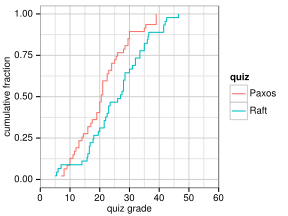
\includegraphics{userstudy/unpairedcdf}
}
\vcaption[quiz score CDF]{
CDF of participants' quiz scores.
Each curve shows the fraction of participants who scored at most
that many points (right/lower is better); for example, about 47\% of
participants scored up to 25 points on the Raft quiz; the remaining 53\%
scored higher.
The maximum possible score was \SI{60}{points} on each quiz.
47 participants completed the Paxos quiz; 45 completed the Raft quiz.
Figure~\ref{fig:userstudy:diffBreak} facets this graph down by question
difficulty and ordering.
}
\label{fig:userstudy:unpairedcdf}
\end{figure}

Figure~\ref{fig:userstudy:unpairedcdf} shows the raw distributions of quiz scores;
the Raft scores are generally greater than the Paxos scores by
a few points.
The mean Raft score is \SI{4.74}{points} or 22.6\% higher than
the mean Paxos score.
We used a statistical significance test to confirm this difference:
we conducted an unpaired Student's \emph{t}-test with a one-sided
hypothesis that the Raft scores were greater than the Paxos scores.
This test found that
the Raft scores (\emph{M}~=~25.72, \emph{SD}~=~10.33) were significantly
greater than the Paxos scores (\emph{M}~=~20.98, \emph{SD}~=~8.57);
\emph{t}(85.55)~=~2.39, \emph{p}~=~0.009.
In layman's terms, we can say with 99\%
confidence from our sample that the true distribution of Raft quiz
scores is greater than the true distribution of Paxos quiz scores
(there is only a 1\% chance that we would find such a difference by
random chance in identical distributions; a $p$-value less than 5\%
is typically considered statistically significant).

\begin{figure}
\centering
{
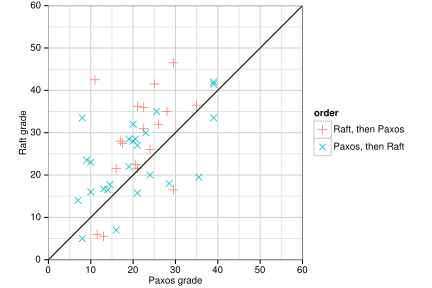
\includegraphics{userstudy/pairedscatter}
}
\vcaption[quiz score scatter plot (by school)]{
A scatter plot of 43 participants' grades comparing their performance on
each quiz. Points above the diagonal (33) represent participants who
scored higher on the Raft quiz.
The shape and color of each point represent whether that particular
participant watched the Raft lecture and took the Raft quiz first or
whether he/she watched the Paxos lecture and took the Paxos quiz first.
Figure~\ref{fig:userstudy:pairedscatterpaxos} is a similar scatter plot which
shows participants' prior Paxos exposure instead.
}
\label{fig:userstudy:pairedscatter}
\end{figure}

\begin{figure}
\centering
{
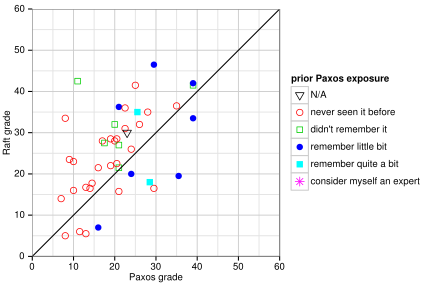
\includegraphics{userstudy/pairedscatterpaxos}
}
\vcaption[quiz score scatter plot (by prior Paxos exposure)]{
A scatter plot of 43 participants' grades comparing their performance on
each quiz, showing the participants' prior Paxos exposure.
The shape and color of each point represent the prior Paxos exposure
that participant reported in the survey
(the exact question can be found in
Appendix~\ref{appendix:userstudy:survey}). One participant did not
respond to the question (labeled ``N/A'').
No students reported prior Raft exposure.
Figure~\ref{fig:userstudy:pairedscatter} is a similar scatter plot which
shows the order in which participants took the quizzes instead.
}
\label{fig:userstudy:pairedscatterpaxos}
\end{figure}

\begin{figure}
\centering
{
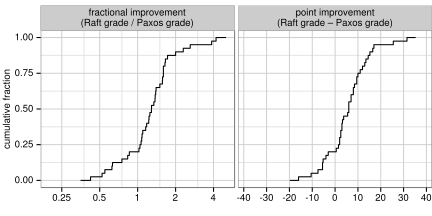
\includegraphics{userstudy/pairedcdf}
}
\vcaption[CDF of participants' quiz score difference]{
CDF of 43 participants' Raft scores compared to their Paxos scores.
The left graph shows participants' relative score difference between the
quizzes (an $x$-value of 2 means the participant's score on the Raft
quiz was twice their score on the Paxos quiz).
The right graph shows the participants' absolute score difference
between the quizzes (positive values represent participants who scored
higher on Raft).
}
\label{fig:userstudy:pairedcdf}
\end{figure}

We also wanted to consider individual differences in learning and
test-taking abilities. Because participants learned and took quizzes
on both algorithms, we could look at each participants' difference in
quiz scores. (Six participants only took one quiz, so we exclude them
here.)

Figures~\ref{fig:userstudy:pairedscatter} and \ref{fig:userstudy:pairedscatterpaxos} plot
individuals' quiz scores against each other. They show that 33 of 43 of
the participants scored higher on their Raft quiz than on their Paxos
quiz. Figure~\ref{fig:userstudy:pairedscatter} overlays the order in which
participants learned the algorithms and took the quizzes, while
Figure~\ref{fig:userstudy:pairedscatterpaxos} overlays participants' prior Paxos
exposure. Neither of these appear to be obviously correlated with which
participants scored higher on their Raft quiz.

Figure~\ref{fig:userstudy:pairedcdf} shows the overall distribution of
how participants scores differ across exams; this makes it easier to
compare the overall behavior of the data.
The participants' scored a median of \SI{6.5}{points} or
31.7\% higher on
the Raft quiz than on the Paxos quiz.
We conducted a paired samples \emph{t}-test with a one-sided
hypothesis that participants Raft scores were generally greater than
their Paxos scores.
This test found that
individuals' Raft scores (\emph{M}~=~25.73, \emph{SD}~=~10.56) were
significantly
greater than their Paxos scores (\emph{M}~=~20.79, \emph{SD}~=~8.64);
\emph{t}(42)~=~3.39, \emph{p}~=~0.001.
In layman's terms, we can say with 99.9\%
confidence from our sample that similar individuals will
score greater on their Raft quiz than on their Paxos quiz
(there is only a 0.1\%
chance that we would find such a difference by
random chance in identical distributions).

\begin{figure}
\centering
{
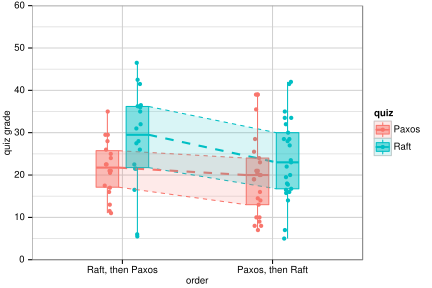
\includegraphics{userstudy/order}
}
\vcaption[ordering effects]{
Ordering effects on participants' quiz scores.

The boxplots summarize the participants' quiz score distributions. The
top of each line is the maximum score attained, the top of each box is
the $\mathrm{75}^\mathrm{th}$ percentile, the middle of each box is the
median, the bottom of each box is the $\mathrm{25}^\mathrm{th}$
percentile, and the bottom of each line is the minimum score attained.

Dashed lines connect the quantiles on boxplots for the same quiz between
different ordering groups. For example, the thick, dashed, blue line
connects the median score for the Raft quiz in the group that took the
Raft quiz first (left) to the median score for the Raft quiz in the
group that took the Raft quiz second (right). If the ordering of the
quizzes did not affect participants' performance, these dashed lines would
be nearly horizontal.

Participants' individual quiz scores overlay each boxplot to provide
further detail. Each point's \emph{x} coordinate is randomly offset to
reduce overlap.
}
\label{fig:userstudy:order}
\end{figure}

We were also curious whether the order in which students learned the systems
affected their quiz scores.
Figure~\ref{fig:userstudy:order} shows participants' quiz scores grouped by
whether they took the Raft quiz first or second.
It appears from the figure that the participants who took the Raft quiz
first scored about five points higher on the Raft quiz than those who
took the Paxos quiz first.
To investigate this effect, we used statistical tests to determine
whether the scores in the two groups truly differed for the same quiz:
we conducted
unpaired \emph{t}-tests with two-sided hypotheses that the groups
differed in either direction.
These showed no statistically significant differences between
the groups; such a difference for Raft could occur by random
chance in 16.8\% of similar experiments.
However, ordering does appear to be a statistically significant factor
when also considering prior Paxos experience; this is discussed next as
a component of a linear regression model.

We created a linear regression model to investigate the effects of various factors
on quiz scores. The model considered whether the participants were
taking their first or second quiz, their prior Paxos experience, and
their school. To test whether ordering and prior Paxos experience
affected the Raft or Paxos quizzes differently, the linear model
included two variables for each of those. Thus, the model included the
following variables:
\begin{compactitem}
\item \textbf{Quiz:} Paxos or Raft.
\item \textbf{Second quiz, Raft:} the participant took the Paxos quiz before
the Raft quiz, and \emph{Quiz} is Raft.
\item \textbf{Second quiz, Paxos:} the participant took the Raft quiz before
the Paxos quiz, and \emph{Quiz} is Paxos.
\item \textbf{Prior Paxos experience, Raft:}
the participant's prior Paxos experience if the \emph{Quiz} is Raft,
0 otherwise. In order to include this factor in the model,
participants' prior Paxos experience was mapped from the
English answer labels found in Appendix~\ref{appendix:userstudy:survey}
to integers between 0 and 4.
\item \textbf{Prior Paxos experience, Paxos:}
the participant's prior Paxos experience if the \emph{Quiz} is Paxos,
0 otherwise.
\item \textbf{School:} Stanford or Berkeley.
\end{compactitem}

Our first model (Table~\ref{tab:userstudy:lm1}) reported that the \emph{School}
factor was insignificant, so we created a second model that excludes it.
The second model, shown in Table~\ref{tab:userstudy:lm2}, explains
19\% of the
variance in quiz scores; the other 81\% at least includes individual
differences in learning and test-taking abilities. Accounting for
ordering, this model predicts quiz scores
that are \SI{12.5}{points} higher on the Raft quiz than on the Paxos quiz for
students with no prior Paxos experience.

\begin{table}
\centering
\begin{tabular}{lrrrr}
variable & estimate & std. error & \emph{t}-value & \emph{p}-value \\
\hline
\noalign{\vskip .75ex}
Intercept                       & $10.61$ & $3.32$ &  $3.19$ & $0.002$ \\
Quiz is Raft                    & $12.99$ & $4.46$ &  $2.92$ & $0.005$ \\
Second quiz, Raft               & $-6.74$ & $2.87$ & $-2.35$ & $0.021$ \\
Second quiz, Paxos              &  $4.09$ & $2.87$ &  $1.42$ & $0.158$ \\
Prior Paxos experience, Paxos   &  $4.65$ & $1.54$ &  $3.02$ & $0.003$ \\
Prior Paxos experience, Raft    &  $3.11$ & $1.54$ &  $2.02$ & $0.046$ \\
School is Berkeley              &  $3.26$ & $2.28$ &  $1.43$ & $0.157$
\end{tabular}


\vcaption[linear model of quiz grades, including school factor]{
Linear model of quiz grades, including school factor.
This model is statistically significant (F(6,77)~=~4.48, p~=~0.001). It
explains 20\% of the variance in quiz scores (adjusted
$\textrm{R}^\textrm{2}$~=~0.20).
\\
The ``Intercept'' represents a constant number of points predicted as a
baseline for every participant. The value of each variable is multiplied
by its coefficient in the ``Estimate'' column; these are summed to form
the predicted quiz score. For example, a Berkeley student taking her
Raft quiz after having taken her Paxos quiz, with no prior Paxos
experience, would be expected to receive a quiz score of
$10.61 + 12.99(1) - 6.74(1) + 4.09(0) + 4.65(0) + 3.11(0) + 3.26(1) = 20.12$.
The ``\emph{p}-value'' represents the probability that each
variable's co-efficient does not significantly differ from 0; normally
\emph{p}-values below 0.05 are considered statistically significant.
The ``Std. Error'' and ``\emph{t}-value'' columns are used to calculate
the \emph{p}-values.
\\
Two variables in this model are not statistically significant:
``Second Quiz, Paxos'' and ``School is Berkeley''.
In refining this model to arrive at Table~\ref{tab:userstudy:lm2},
we kept the
``Second Quiz, Paxos'' variable because it is symmetric with the
``Second Quiz, Raft'' variable, which is significant. However, we
dropped the ``School is Berkeley'' variable.
}
\label{tab:userstudy:lm1}
\end{table}

\begin{table}
\centering
\begin{tabular}{lrrrr}
variable & estimate & std. error & \emph{t}-value & \emph{p}-value \\
\hline
\noalign{\vskip .75ex}
Intercept                       & $11.27$ & $3.31$ &  $3.40$ & $0.001$ \\
Quiz is Raft                    & $12.54$ & $4.74$ &  $2.80$ & $0.006$ \\
Second quiz, Raft               & $-6.30$ & $2.87$ & $-2.19$ & $0.031$ \\
Second quiz, Paxos              &  $3.64$ & $2.87$ &  $1.27$ & $0.209$ \\
Prior Paxos experience, Paxos   &  $4.88$ & $1.54$ &  $3.18$ & $0.002$ \\
Prior Paxos experience, Raft    &  $3.35$ & $1.54$ &  $2.18$ & $0.032$
\end{tabular}
\vcaption[linear model of quiz grades, excluding school factor]{
Linear model of quiz grades, excluding school factor.
This model is statistically significant (F(5,78)~=~4.90, p~=~0.0006). It
explains 19\% of the variance in quiz scores (adjusted
$\textrm{R}^\textrm{2}$~=~0.19).
}
\label{tab:userstudy:lm2}
\end{table}

The linear model also predicts higher scores on both quizzes for people
who learn Raft before Paxos (\SI{6.3}{points} on the Raft quiz and
\SI{3.6}{points}
on the Paxos quiz). This difference is statistically significant for
the Raft quiz (p~=~0.031) but not for the Paxos quiz (p~=~0.209). We
speculate that learning Paxos first may have confused or discouraged our
participants enough that they then performed worse on the Raft quiz.

\begin{figure}
\centering
{
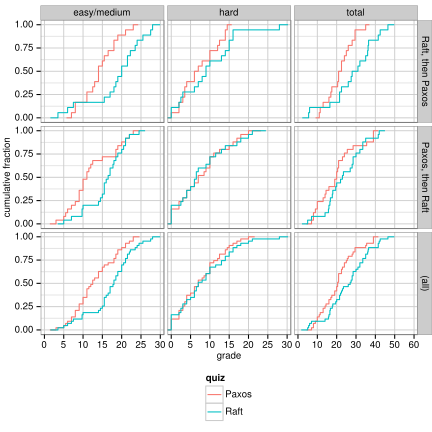
\includegraphics{userstudy/diffBreak}
}
\vspace{-4ex}
\vcaption[quiz score CDFs by question difficulty and ordering]{
CDFs of 43 participants' quiz scores, broken down by question difficulty
and ordering. 
Each curve shows the fraction of participants who scored up to
that many points (right/lower is better).
The \emph{total}, \emph{(all)} graph is
identical to Figure~\ref{fig:userstudy:unpairedcdf}.

\textbf{Difficulty:}
The \emph{easy/medium} column shows the participants' scores for the easy and
medium questions on the quiz, out of a maximum possible \SI{30}{points}.
The \emph{hard} column shows the participants' scores for the hard
questions on the quiz, out of a maximum possible \SI{30}{points}.
The \emph{total} column shows the participants' total scores, out of a
possible \SI{60}{points}.
Figure~\ref{fig:userstudy:breakdown} breaks this down by individual question.

\textbf{Ordering:}
The \emph{Raft, then Paxos} row shows the scores for the
participants who took the Raft quiz before taking the Paxos quiz.
The \emph{Paxos, then Raft} row shows the scores for the
participants who took the Paxos quiz before taking the Raft quiz.
The \emph{(all)} column shows the scores for all participants who took
both quizzes.
}
\label{fig:userstudy:diffBreak}
\end{figure}

Figure~\ref{fig:userstudy:diffBreak} shows distributions of quiz scores broken
down by question difficulty. There were only \SI{4}{points} of Easy questions,
so we combined those with the Medium category in the graphs.
The graphs show that almost all of the difference
in scores can be attributed to questions in the Easy/Medium category,
and the Hard category accounted for only a very small difference in
scores. We made the hard questions too difficult: on average,
participants scored only about one quarter of the possible points in the
Hard category (\SI{7.45}{points} on average on Paxos and
\SI{7.94}{points} on
average on Raft). Thus, we were unable to measure much difference
between participants in the Hard category.

\begin{figure}
\centering
{
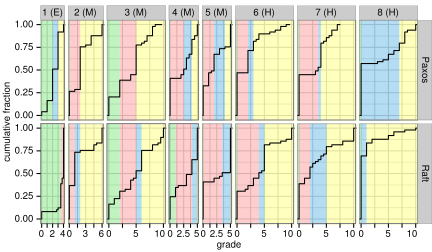
\includegraphics{userstudy/breakdown}
\vspace{-1ex}\\
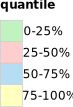
\includegraphics{userstudy/breakdownlegend}
}
\vcaption[quiz score CDFs by question]{
CDFs of participants' scores on individual questions.

Each graph in the figure shows the quiz scores for an individual quiz
question. The top row of graphs shows Paxos quiz questions; the bottom
row shows Raft quiz questions. The number above each graph is the number
of the question (multi-part questions have been aggregated to save
space).

The curve in each graph shows a CDF of the data. The
\emph{y} axis is the cumulative fraction of participants who scored up
to a given number of points (right/lower is better).

The range of the \emph{x} axis on each graph corresponds to the
point values possible for each question, and one point has the same width
in every graph. For example, the graph for a 10-point question is twice
as wide as the graph for a 5-point question.

Each graph is also colored to provide summary information at a glance.
Each quantile of the data is shaded in a different color, as shown
in the legend. Because each graph's width is scaled to its point value,
the size (area) of the shading is proportional to the number of points
it represents.
}
\label{fig:userstudy:breakdown}
\end{figure}

Figure~\ref{fig:userstudy:breakdown} breaks the quiz scores down by individual
question. Question 1 was Easy difficulty, Questions 2 through 5 were
Medium difficulty, and Questions 6 through 8 were Hard difficulty, based
on our categorization. There do not appear to be any individual
questions in the Medium category that alone account for large
differences. Although we tried to pair question difficulty across
quizzes (for example, Q3 on the Raft quiz should be about as difficult
as Q3 on the Paxos quiz), they are mostly different questions that are
hard to compare directly.

\subsection{Survey}
\label{userstudy:results:survey}

Participants answered three groups of survey questions after taking their
second quiz.
The questions asked
about their prior experience with Paxos and Raft,
whether they felt the lectures or quizzes were biased, and which
algorithm they felt would be easier to implement or explain.
Participants were also asked for open-ended comments or feedback.
The full survey and exact questions can be found in
Appendix~\ref{appendix:userstudy:survey}, along with the open-ended
comments and feedback.

\begin{figure}
\centering
{
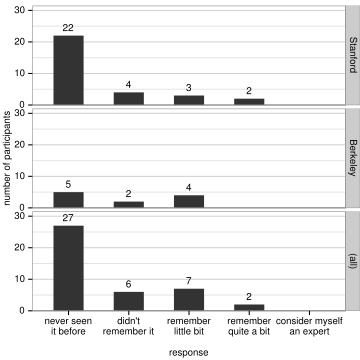
\includegraphics{userstudy/surveypaxos}
}
\vcaption[prior Paxos experience survey]{
Prior Paxos experience survey.
Using a five-point scale, participants were asked how much prior exposure
they had to Paxos; 42 participants responded to the question.
The top graph shows the responses from the Stanford participants, the
middle graph shows the responses from the Berkeley participants, and the
bottom graph shows the total responses (from all participants).
}
\label{fig:userstudy:surveypaxos}
\end{figure}

Many of the Berkeley participants and some of the Stanford participants
had prior exposure to Paxos; Figure~\ref{fig:userstudy:surveypaxos} shows
their responses to the survey question. At Stanford, 9 of the 31
participants who responded to the question had at least some prior
exposure to Paxos. At Berkeley, 6 of the 11 participants who
responded to the question had at least some prior exposure to Paxos.
No participants reported any prior exposure to Raft (41 participants
responded to this question); Raft was still new at the time, so this was
expected.

\begin{figure}
\centering
{
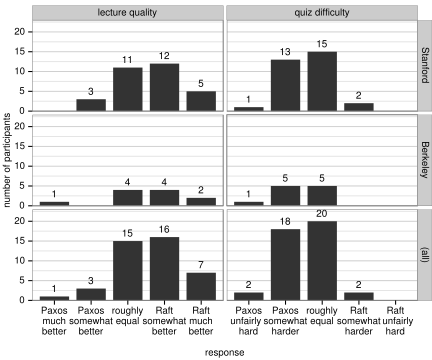
\includegraphics{userstudy/surveyfair}
}
\vcaption[fairness survey]{
Fairness survey.
Using a five-point scale, participants were asked which lecture was better
and which quiz was more difficult.
42 participants responded to each question.
\\
\textbf{Left:}
Do you think the video lectures were roughly equal in quality, given the
nature of the material being presented?
\\
\textbf{Right:}
Do you think the quizzes were roughly equal in terms of testing your
understanding of the material?
\\
The top graphs show the responses from the Stanford participants, the
middle graphs show the responses from the Berkeley participants, and the
bottom graphs show the total responses (from all participants).
}
\label{fig:userstudy:surveyfair}
\end{figure}

Participants were also asked whether they felt the lectures were of
similar quality and whether the quizzes were of similar difficulty;
Figure~\ref{fig:userstudy:surveyfair} shows their responses.
23 of 42 participants responded that the Raft lecture was at least
somewhat better than the Paxos lecture, and 20 of 42 participants
responded that the Paxos quiz was at least somewhat harder than the Raft
quiz.
However, these responses may be unreliable: it may have been difficult
for participants to separate
the intrinsic difficulty of the material or
their level of understanding from the
lecture quality, or their performance from the quiz difficulty.
Therefore, we do not consider this strong evidence against the integrity
of our study.

\begin{figure}
\centering
{
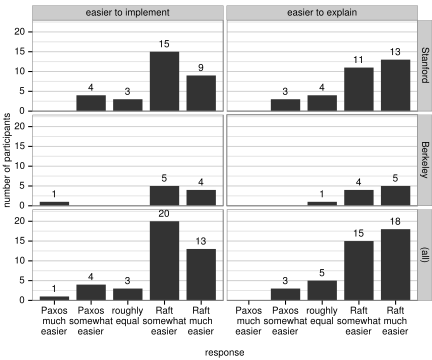
\includegraphics{userstudy/survey}
}
\vcaption[preferences survey]{
Preferences survey.
Using a five-point scale, participants were asked which algorithm would be
easier to implement and which would be easier to explain.
41 participants responded to each question.
\\
\textbf{Left:}
Suppose you were working at a company and it is your job to implement a
replicated state machine. Which algorithm would be easier to implement in a
functioning, correct, and efficient system?
\\
\textbf{Right:}
Suppose you had to explain either Raft or Paxos to a CS graduate student who
hadn't seen either one previously. Which would be easier to explain?
\\
The top graphs show the responses from the Stanford participants, the
middle graphs show the responses from the Berkeley participants, and the
bottom graphs show the total responses (from all participants).
}
\label{fig:userstudy:survey}
\end{figure}

Figure~\ref{fig:userstudy:survey} shows which algorithms participants felt would
be easier to implement or explain. An overwhelming majority of
participants preferred Raft for each: 33 of 41 participants reported
that Raft would be at least somewhat easier to implement, and 33 of 41
participants reported that Raft would be at least somewhat easier to
explain.
However, these self-reported feelings may
be less reliable than participants' quiz scores, and participants may
have been biased by knowledge of our hypothesis that Raft is easier to
understand.

%


\section{Discussion about the experimental approach}
\label{userstudy:approachdiscussion}

Initially, we doubted that a user study would be feasible or convincing,
but we felt it was the most appropriate way to evaluate Raft's claim of
understandability. Thus, we conducted the user study to provide
empirical evidence that Raft is easier to understand than Paxos.
Although we consider the study itself successful, it
was not particularly well-received by the system community.
This section explores whether the study was
worth the time and effort we put into it and sheds light into whether
this sort of experiment is effective in the systems community.

In our first paper submission on Raft (in 2012),
we claimed the Raft algorithm was
easier to understand than Paxos, but we had essentially no objective
evidence for this. Our anonymous reviewers rightly pointed out this
weakness. Excerpts from their reviews serve as evidence that with no
evaluation, our claim of understandability was weak:
\begin{itemize}
\em
\item It's not clear Raft is any more understandable than Paxos. While
understandability is the key claim to novelty, this claim was not
actually evaluated, and may be untrue.\ \ldots\ 
I think one thing that would have helped a lot is if the authors chose a
concrete ``metric of success'' and evaluated their system according to
that metric.\ \ldots\ 
I do like the idea of using understandability as a metric, but that [sic]
there was no attempt at all to actually characterize Raft using that
metric.

\item
\ldots\ I understood the algorithm. So, perhaps that speaks to the fact
that Raft is indeed understandable.

That said, I do think that you [need] a way to show that Raft is indeed
more understandable. A couple of thoughts on doing that:

\begin{compactitem}
\item Compare implementations of Raft and Paxos using some code
complexity measures.
\item Explain Raft and Paxos to students, and see which one they
understand better. A test of understanding could be writing the
pseudocode, a quiz on algorithm behavior, or extending the algorithm to
do something different.
\end{compactitem}

\item We encourage the authors to define metrics for
``understandability'' and systematically explore whether the protocol
meets these goals.\ \ldots
\end{itemize}


Based of this feedback, we conducted the Raft user study and included
its results in our second paper submission. Unfortunately, the study did
not seem to convince most of our reviewers; they did not seem to find
much value in it. Several did not even mention it in their reviews.
Others were concerned about the lecture content and quiz questions, even
though we referred our readers to the user study lectures and quizzes
online. The paper was ultimately accepted (in 2014) after several attempts, but
we feel this was despite the reviewers' generally negative opinions of
the study. The following excerpts summarize the reviewers' opinions
about the user study:

\begin{itemize}
\em


\item The user study is not that useful.

\item The evaluation is thin.  Its qualitative thesis (Raft is simpler
$\Rightarrow$ Raft is more understandable $\Rightarrow$ Raft
implementations are more correct) is poorly supported, and hence subject
to the reader's counter intuition.\ \ldots\ 
This paper's evaluation hinges on the user study. Did the tests test the
corner cases? Did the students have to prove either system correct,
formally?

\item I'm disappointed that Section 7 [Clients and log compaction] is
empty! Given a choice, I'd rather omit Section 8 [Implementation and
evaluation] and include Section 7.

\item The user study is a nice idea, but ultimately I don't think it
adds much to the paper. Readers will decide for themselves if the
algorithm is understandable or not and the paper's ultimate impact will
depend on this judgement, not a user study.



\item The user study is interesting.

Unclear whether explaining Paxos more clearly would change the
results of the user study.

\item Reasonable user study about ``understandability''.

User study, while laudable, seems fairly unscientific in the end due
to potential large sources of bias.

I appreciate the author's attempts to better characterize
whether Raft is indeed ``more understandable'' than Paxos, and care was
put into designing the study (e.g., splitting users, presenting them
with tests is different orders, etc.).  Even so, if our goal is really
randomized trials, the fact that the experimenters wrote the
explanations of the two protocols gives me some real pause about some
pretty overt bias that could slip into the writeup.

\item User study is fresh and interesting (albeit bias factors are present).

The user study is interesting and thought provoking, but it really lacks
representativeness both in terms of sample sizes as well as neutrality.

\item I think the understandability study is interesting, but perhaps a
little bit of overkill.  Typically researchers can compare two protocols
and see for themselves which is simpler \ldots
But I'm not against a little overkill now and then.  However,
summarizing a study with a statement such as ``students were able to
answer questions about Raft 23\% better than questions about Paxos''
raises immediate questions about whether such figure is very meaningful.
In particular 23\% seems like a precise figure, but in fact depends a lot
on how the tutorials and the test are set up (even when strong measures
are taken to ensure fairness, as you have done).  Two issues that come
to mind are that you can't ask exactly the same questions about two
different protocols, and even if you could, it's not clear which
questions would be the right or fair questions to ask to get at the
issue of understandability.

\item The user study based on self-reported understandability scores and
correctness of answering problem questions is not particularly
convincing. It would be more convincing if students were made to
implement both Paxos and Raft in code, and then compare objectively the
time taken, the lines of code, and the overall correctness.

Concrete suggestion: Please provide some objective measure on
understandability, even if it is for a small sample-set of students that
implement both Paxos and Raft from just communication primitives.



\item I found the sample size in the section on understandability to be
small enough to be worrisome in spite of the good t-test number.  A
better test might be the number of unaccounted for failure modes in
na\"ive implementations.  I expect Raft to win by a wide margin.

\item 
Furthermore, a review of the teaching materials in~\cite{study} seems to
indicate flaws in the way the ``Understandability study'' was
performed. Some implementations of Multi-Paxos support concurrent
proposals which are ordered by the leader. However, it is unclear how
Raft does the same. From the description in the paper, I think Raft
handles Append entries (performing Append RPCs) sequentially. So,
aren't you comparing the understandability of 2 algorithms with
different properties?

\item I find the evaluation of using students' feedback interesting.
However, it's hard to be convinced of your conclusion if I don't know
what quizzes are being asked.

\item The authors evaluation of the subjective claim of
understandability was done valiantly in section 8.1 [Understandability],
bravo.

\item We [reviewer and students] didn't like the user study. It's not
necessary or convincing. Adding more information to make it convincing
would not be worth the space cost.

\end{itemize}

Moreover, conducting the Raft user study was inherently costly and risky
in terms of time and effort. Typically, systems papers evaluate their
performance quantitatively through machine experiments; such experiments
have low cost and fast turnaround. This results in several attractive
properties as compared to psychology experiments involving human
subjects:
\begin{itemize}
\item \textbf{Repeatability:} Performance evaluations are typically
easy and cheap to repeat. They are often automated so that there is
little room for experimenter error in repeating the experiment. On the
other hand, psychology experiments require much more human involvement
in general, making them more costly and more error-prone to repeat.
\item \textbf{Iteration:} Easily repeatable experiments make it possible
to change the system, its environment, or the experiment based on
experimental results. For example, a researcher might discover a bug
during performance evaluation, fix it, and rerun the experiments, at
little or no additional cost. This can be prohibitively costly in a psychology
experiment, as it requires restarting the entire study with a new group
of participants.
\item \textbf{Incremental results:} In a user study, almost all of the
work must be done before seeing any results, or even learning whether
the basic idea makes sense. This makes such experiments much riskier
than performance evaluations, where initial coarse-grained results are
often attainable with little effort.
\end{itemize}

On the other hand, novel approaches can bring some of these properties
to human subjects psychology experiments. For example in one study, Dow
\emph{et al.}~\cite{Dow:2010} compare ad impressions using web
analytics. This is objective, repeatable, allows iteration, and is
incremental. Similar techniques may apply to evaluating
understandability in some domains. Massive open online courses (MOOCs)
may also be a useful experimental platform for understandability by
providing researchers with pools of thousands of students to teach and
evaluate.


Despite reviewers' concerns, we consider the user study to be an
essential part of this work. Its results are the only objective evidence
we have that Raft is easier to understand than Paxos. The results assume
that the study's lectures are of equal quality and that its quizzes are
of equal difficulty. Though we have no way to prove this, the methods
aimed to produce equivalent lectures and quizzes, and the materials are
available for readers to review. Under this assumption, the results
should be convincing, even to skeptical readers.


\section{Conclusion}

The Raft user study compared Raft's understandability to that of Paxos.
The study showed that after learning Paxos or Raft for an hour,
students are able to answer equally difficult questions about Raft
better than they can about Paxos. We believe we countered all major
sources of bias in our study, and the study showed the major result we
wanted. However, it took significant time and effort. We hope future
techniques, such as leveraging online courses, allow studies to achieve
similar results at a lower cost.

The Raft user study was unconventional for systems research, which tends
to focus on machine-based performance evaluations. Our study provides
substantial evidence in favor of Raft's understandability, and as far as
we know, it is the first study to objectively evaluate consensus
algorithms based on teaching and learning. We believe the systems
community should carefully consider such studies, as they enable us to
advance our collective knowledge through novel kinds of contributions
that we could not otherwise convincingly evaluate.
